\subsection{Repositorio}

El notebook \texttt{.ipynb} así como los demás archivos de la práctica se
encuentran en el siguiente repositorio de GitHub:
\hyperlink{P3}{\textcolor{iimasorange}{https://github.com/Garp02/Reconocimiento-Patrones/tree/main/P3}}

\needspace{4\baselineskip}

\subsection{Conjunto de datos y reformulación del problema}

Se trabajó con el conjunto \textbf{Arrhythmia} del \textit{UCI Machine Learning
    Repository}, que contiene 452 registros y 279 características derivadas de
electrocardiogramas (ECG) más una etiqueta de clase. La clase original
distingue entre 16 categorías (normal, 14 tipos de arritmia y una clase
residual). Al inspeccionar su distribución se observó que varias clases
contienen apenas 2 a 5 muestras, lo que hace inviable un planteamiento
multiclase con validación robusta.

Por esta razón se reformuló el problema como una clasificación
\textbf{binaria}: clase 1 (normal) frente al resto (arritmia). La proporción
resultante es de 245 frente a 207 registros, prácticamente balanceada (ratio
$0.542$), por lo que no fue necesario aplicar técnicas de sobremuestreo como
SMOTE. La Figura~\ref{fig:distribucion} muestra ambas distribuciones.

\begin{figure}[H]
    \centering
    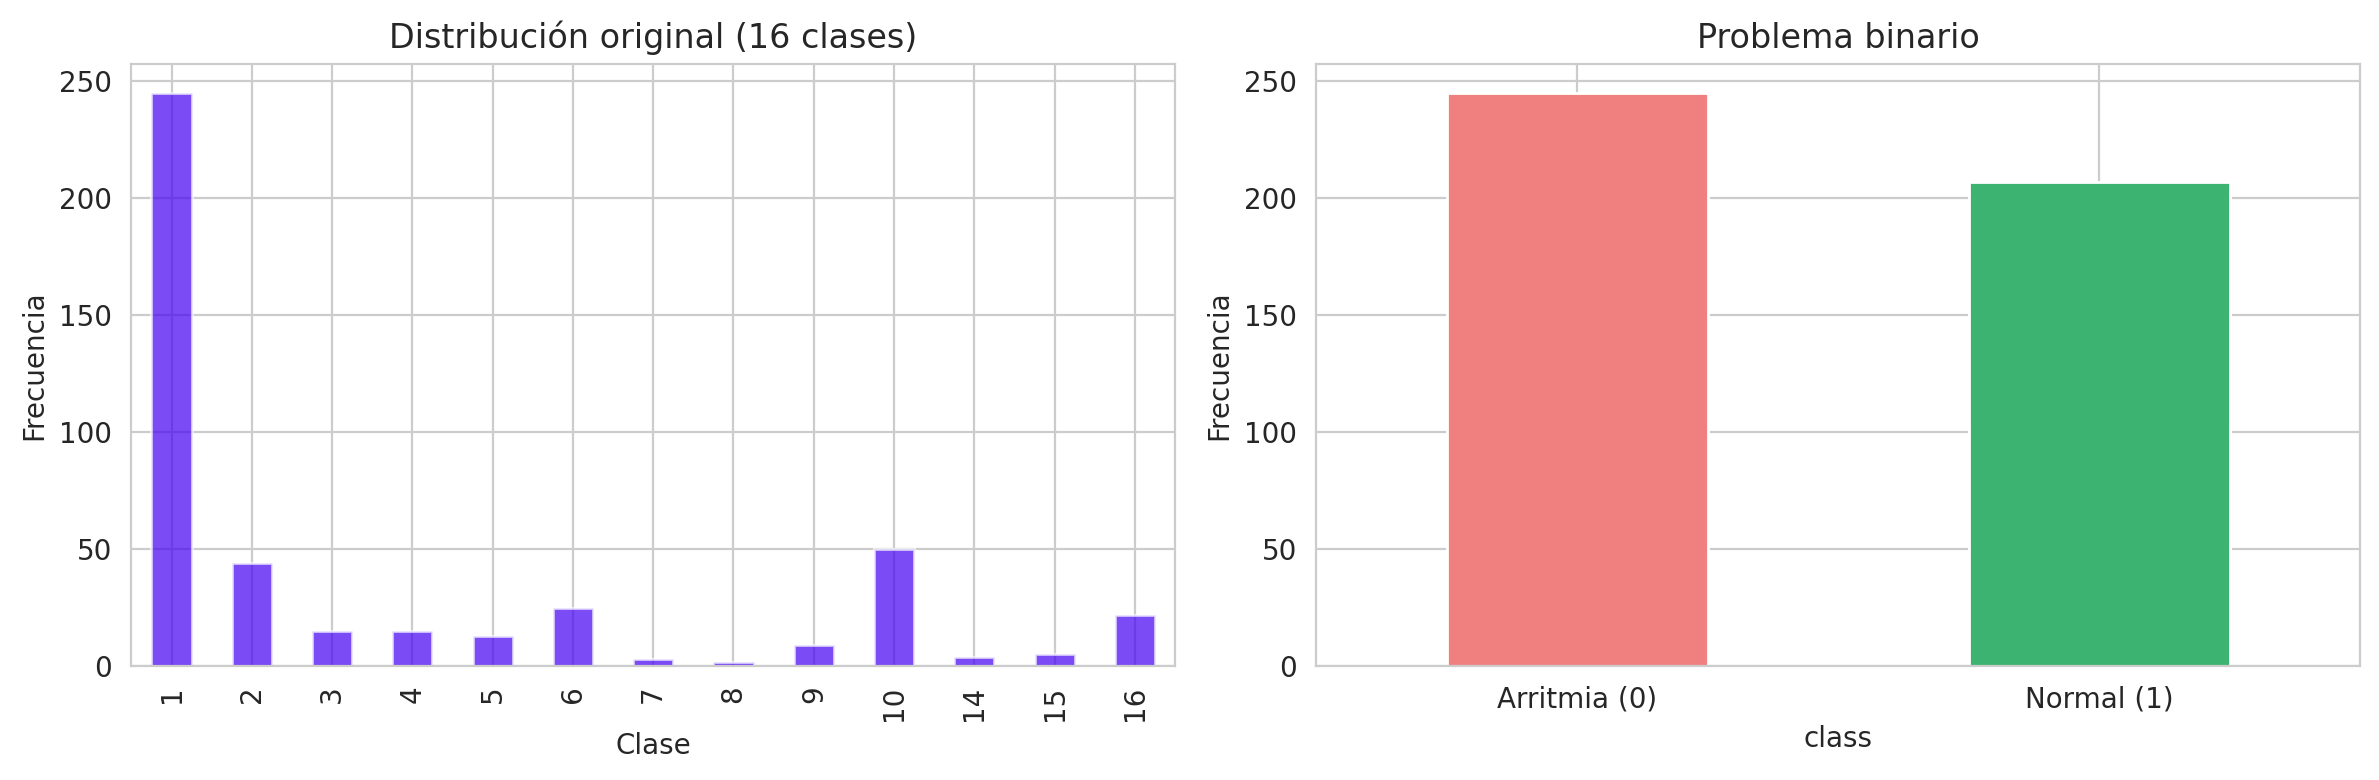
\includegraphics[width = 1\textwidth]{Img/01_distribucion_clases.png}
    \caption{Distribución de clases original (izquierda) y reformulación
        binaria (derecha).}
    \label{fig:distribucion}
\end{figure}

\subsection{Perfilamiento exploratorio con \texttt{ydata\_profiling}}

Como primer diagnóstico se ejecutó \texttt{ydata\_profiling} sobre las 15
primeras columnas (las documentadas en \texttt{arrhythmia.names}: edad, sexo,
medidas antropométricas, duraciones e intervalos del complejo QRS, ángulos
eléctricos y frecuencia cardíaca). Se eligió este subconjunto porque son las
únicas variables con interpretación clínica directa; las restantes 264
corresponden a mediciones derivadas por derivación del ECG cuyo significado
queda implícito.

El reporte general indica las siguientes estadísticas globales:

\begin{itemize}
    \item \textbf{Dimensiones}: 452 observaciones, 15 variables (14 numéricas
          y 1 categórica, \texttt{sex}).
    \item \textbf{Celdas faltantes}: 408 en total, equivalente al $6.0\%$
          del conjunto, concentradas en sólo tres variables.
    \item \textbf{Duplicados}: 0 filas duplicadas.
    \item \textbf{Tamaño en memoria}: 53.1 KiB, $\approx 120$ bytes por
          registro.
\end{itemize}

El informe levantó doce alertas automáticas, agrupables en tres categorías:

\begin{itemize}
    \item \textbf{Valores faltantes.} Tres variables presentan huecos:
          \texttt{j\_angle} con 376 (83.2\%), \texttt{p\_angle} con 22
          (4.9\%) y \texttt{t\_angle} con 8 (1.8\%). La saturación de
          \texttt{j\_angle} hace inviable su imputación sin introducir
          sesgo artificial, por lo que se descartó de forma íntegra. Las
          otras dos, junto con los \texttt{NaN} aislados de
          \texttt{qrst\_angle} y \texttt{heart\_rate}, se imputaron con la
          mediana de la columna en el conjunto de entrenamiento.

    \item \textbf{Correlaciones altas.} El reporte identificó tres pares de
          variables con correlación global fuerte:
          \texttt{heart\_rate}$\leftrightarrow$\texttt{qt\_interval},
          \texttt{p\_interval}$\leftrightarrow$\texttt{pr\_interval} y
          \texttt{qrs\_angle}$\leftrightarrow$\texttt{qrst\_angle}. Todas
          tienen justificación fisiológica: la frecuencia cardíaca acorta
          proporcionalmente el intervalo QT, el intervalo PR engloba al
          intervalo P, y el ángulo QRST se construye a partir del ángulo
          QRS. Este hallazgo es consistente con lo que después se observó
          a escala completa: al aplicar el filtro de $|\rho| > 0.9$ sobre
          las 261 características usables se detectaron 24 pares
          redundantes adicionales.

    \item \textbf{Ceros estructurales.} \texttt{pr\_interval}
          (18 ceros, 4.0\%), \texttt{p\_interval} (12 ceros, 2.7\%) y
          \texttt{qrst\_angle} (6 ceros, 1.3\%). En el contexto clínico,
          un intervalo PR de cero milisegundos no es un valor físico sino
          un código para ``no medible'', típicamente asociado a señales
          donde la onda P está ausente o ilegible. Aunque el dataset no
          documenta explícitamente esta convención, se decidió tratarlos
          como valores válidos para no restar muestras; su efecto se
          mitiga posteriormente con el escalado \textit{z-score}.
\end{itemize}

Adicionalmente se revisaron los rangos de las variables numéricas para
confirmar el problema de escalas heterogéneas: las duraciones (QRS, PR, QT,
T) se miden en milisegundos y rondan valores de 80 a 400; los ángulos
vectoriales oscilan entre $-180^{\circ}$ y $+180^{\circ}$; el peso, la
altura y la edad se expresan en sus unidades naturales; y las 264
características derivadas del ECG (no incluidas en el perfilamiento)
mezclan amplitudes en milivoltios con ángulos y duraciones. Esta
diversidad refuerza la necesidad de estandarizar antes de aplicar métodos
sensibles a la escala como PCA y SVM.

\subsection{Preparación de los datos}

El flujo de preparación aplicado, en este orden, fue el siguiente:

\begin{enumerate}
    \item \textbf{Descartar} la columna \texttt{j\_angle} por su proporción
          de \texttt{NaN} cercana al 83\%.
    \item \textbf{Eliminar} 17 columnas constantes (varianza cero), que no
          aportan información discriminativa.
    \item \textbf{Dividir} los datos de forma estratificada en $80\%/20\%$
          ($n_{train}=361$, $n_{test}=91$). El conjunto de prueba se
          reservó intacto durante toda la experimentación.
    \item \textbf{Imputar} los valores faltantes con la mediana,
          ajustando el imputador solo sobre \textit{train}.
    \item \textbf{Escalar} con \textit{z-score}, nuevamente ajustando
          media y desviación solo en \textit{train} y aplicando la
          transformación a \textit{test}.
\end{enumerate}

Tras estos pasos se conservan \textbf{261 características}. El orden
importa: la partición se realiza antes de imputar y escalar para impedir
que información de \textit{test} contamine la estimación de medianas y
varianzas.

\subsection{Implementación de los métodos}

Como clasificador base para todas las evaluaciones se empleó un \textbf{SVM
    lineal} (\texttt{LinearSVC}, $C=1.0$). La validación cruzada fue $5$-fold
estratificada. El baseline con las 261 características originales alcanzó
una exactitud en CV de $0.6731 \pm 0.0452$.

\subsubsection*{Búsqueda Secuencial hacia delante (SFS)}

El método se aplicó de dos formas, con el fin de comparar una
implementación desde cero contra la de una biblioteca estándar:

\begin{itemize}
    \item \textbf{SFS manual}. Partiendo del conjunto vacío, en cada
          iteración se añade la característica que más eleva la exactitud
          en CV. Se aplicó \textit{early stopping} con paciencia de 3
          iteraciones sin mejora. Este criterio equivale al descrito en
          el enunciado.

    \item \textbf{SFS de \texttt{scikit-learn}}. Se utilizó el estimador
          \texttt{SequentialFeatureSelector} con
          \texttt{n\_features\_to\_select = "auto"} y
          \texttt{tol = $10^{-3}$}. El parámetro \texttt{tol} implementa
          un \textit{early stopping} distinto: se detiene cuando la
          mejora entre dos iteraciones consecutivas es menor a ese
          umbral. A diferencia del criterio de paciencia, esta variante
          se detiene a la primera iteración estancada y por tanto es
          algo más conservadora.
\end{itemize}

La versión manual se detuvo en la iteración 12 tras tres iteraciones sin
mejora, quedándose con las \textbf{9 primeras características} y una
exactitud en CV de $\mathbf{0.7782}$. La versión de \texttt{sklearn}
concluyó con \textbf{7 características} y una exactitud en CV de
$\mathbf{0.7755}$. La Figura~\ref{fig:sfs} sobrepone ambos resultados: la
curva corresponde a la traza iteración a iteración de la versión manual
(único método que expone el historial), mientras que el punto azul marca
el resultado final de \texttt{sklearn}.

\begin{figure}[H]
    \centering
    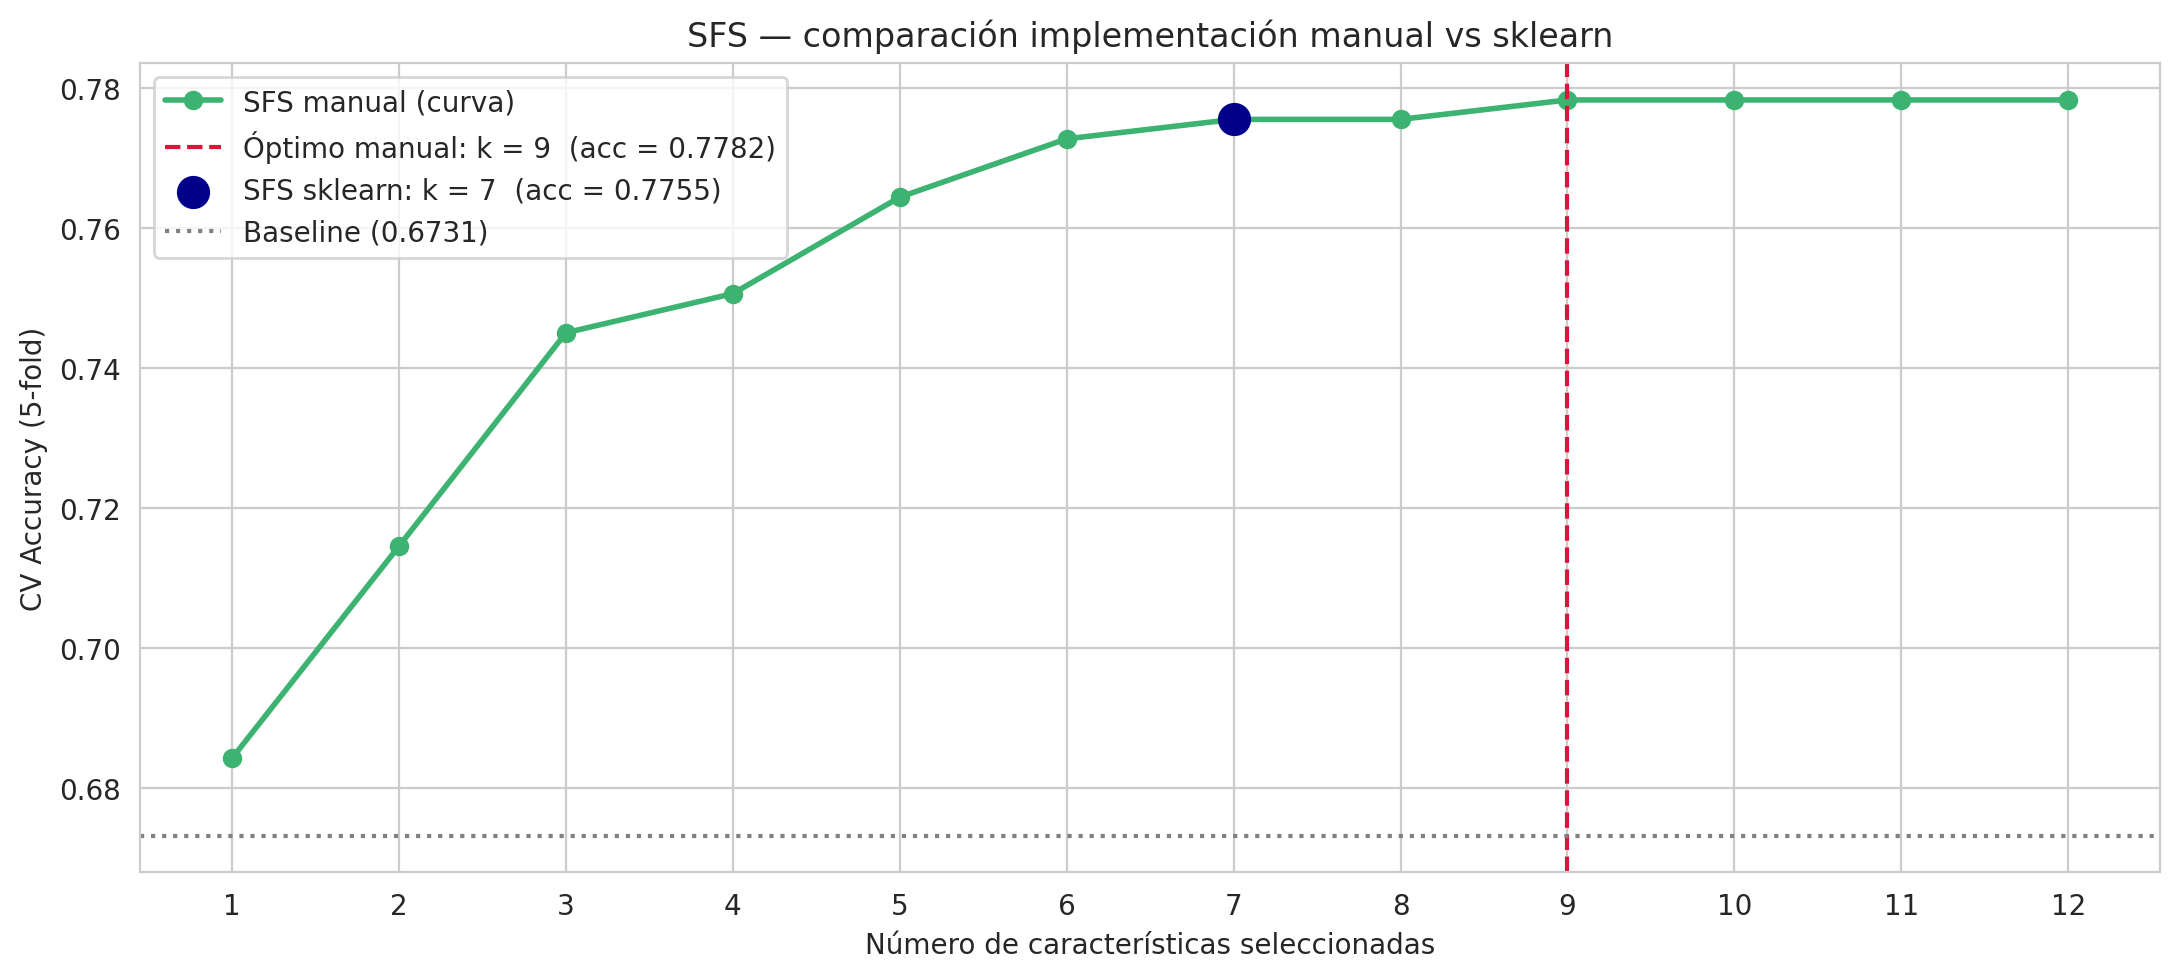
\includegraphics[width=0.9\textwidth]{Img/02_sfs_curva.png}
    \caption{SFS con \textit{early stopping}: curva de aprendizaje de la
        implementación manual y comparación con el resultado de
        \texttt{SequentialFeatureSelector} de \texttt{scikit-learn}.}
    \label{fig:sfs}
\end{figure}

Las 9 características seleccionadas por la versión manual son:
\texttt{qrs\_duration}, \texttt{a\_169}, \texttt{a\_103}, \texttt{a\_114},
\texttt{a\_250}, \texttt{a\_61}, \texttt{a\_44}, \texttt{height} y
\texttt{a\_73}. Las 7 elegidas por \texttt{sklearn} son:
\texttt{qrs\_duration}, \texttt{a\_44}, \texttt{a\_61}, \texttt{a\_103},
\texttt{a\_114}, \texttt{a\_169} y \texttt{a\_250}. La coincidencia es
total: las 7 de \texttt{sklearn} son exactamente un subconjunto de las 9
del método manual, lo que refuerza la estabilidad del núcleo
discriminativo. Las dos características adicionales (\texttt{height} y
\texttt{a\_73}) aportan mejoras marginales que el criterio de
\texttt{sklearn} (sin paciencia) no considera suficientes.

\subsubsection*{Fisher Score}

Para un problema con $C$ clases, la puntuación de Fisher de la característica
$j$ se define como

\begin{equation}
    F_j = \frac{\sum_{c=1}^{C} n_c\,(\mu_j^{(c)} - \mu_j)^2}
    {\sum_{c=1}^{C} n_c\,(\sigma_j^{(c)})^2},
    \label{eq:fisher}
\end{equation}

donde $\mu_j$ es la media global de la característica, $\mu_j^{(c)}$ y
$\sigma_j^{(c)}$ la media y desviación estándar dentro de la clase $c$, y
$n_c$ el número de muestras de esa clase. El numerador mide la varianza
\textit{entre clases} y el denominador la varianza \textit{intra-clase}.
Valores altos indican mayor separabilidad.

Los 20 atributos con mayor puntuación de Fisher se muestran en la
Figura~\ref{fig:fisher-ranking}. La característica más discriminativa es
\texttt{qrs\_duration} ($F \approx 0.14$), coincidente con la primera
elegida por ambas versiones de SFS. La curva de la
Figura~\ref{fig:fisher-topk} indica cómo varía la exactitud al usar los
$k$ mejores atributos.

\begin{figure}[H]
    \centering
    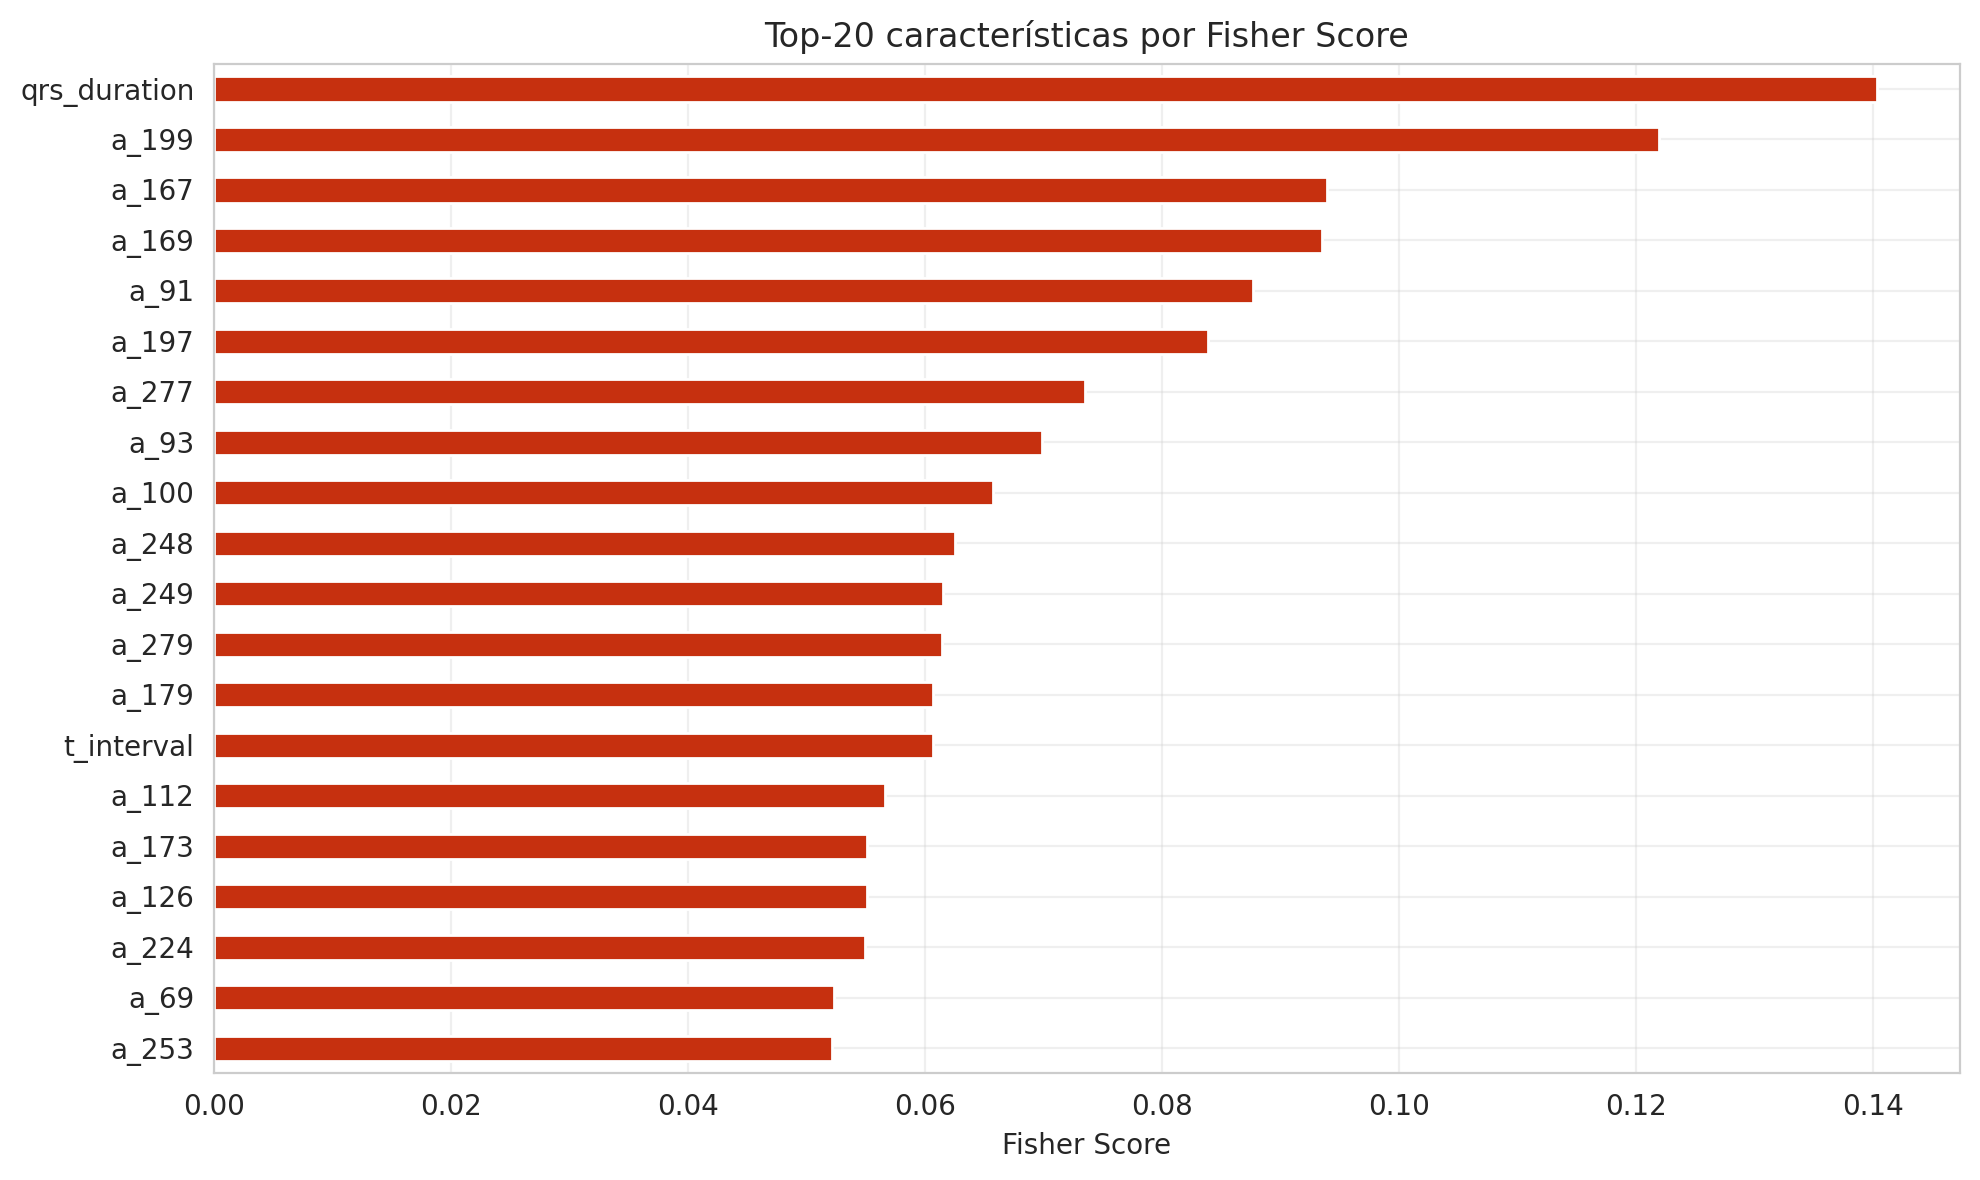
\includegraphics[width=0.85\textwidth]{Img/03_fisher_ranking.png}
    \caption{20 características con mayor Fisher Score.}
    \label{fig:fisher-ranking}
\end{figure}

\begin{figure}[H]
    \centering
    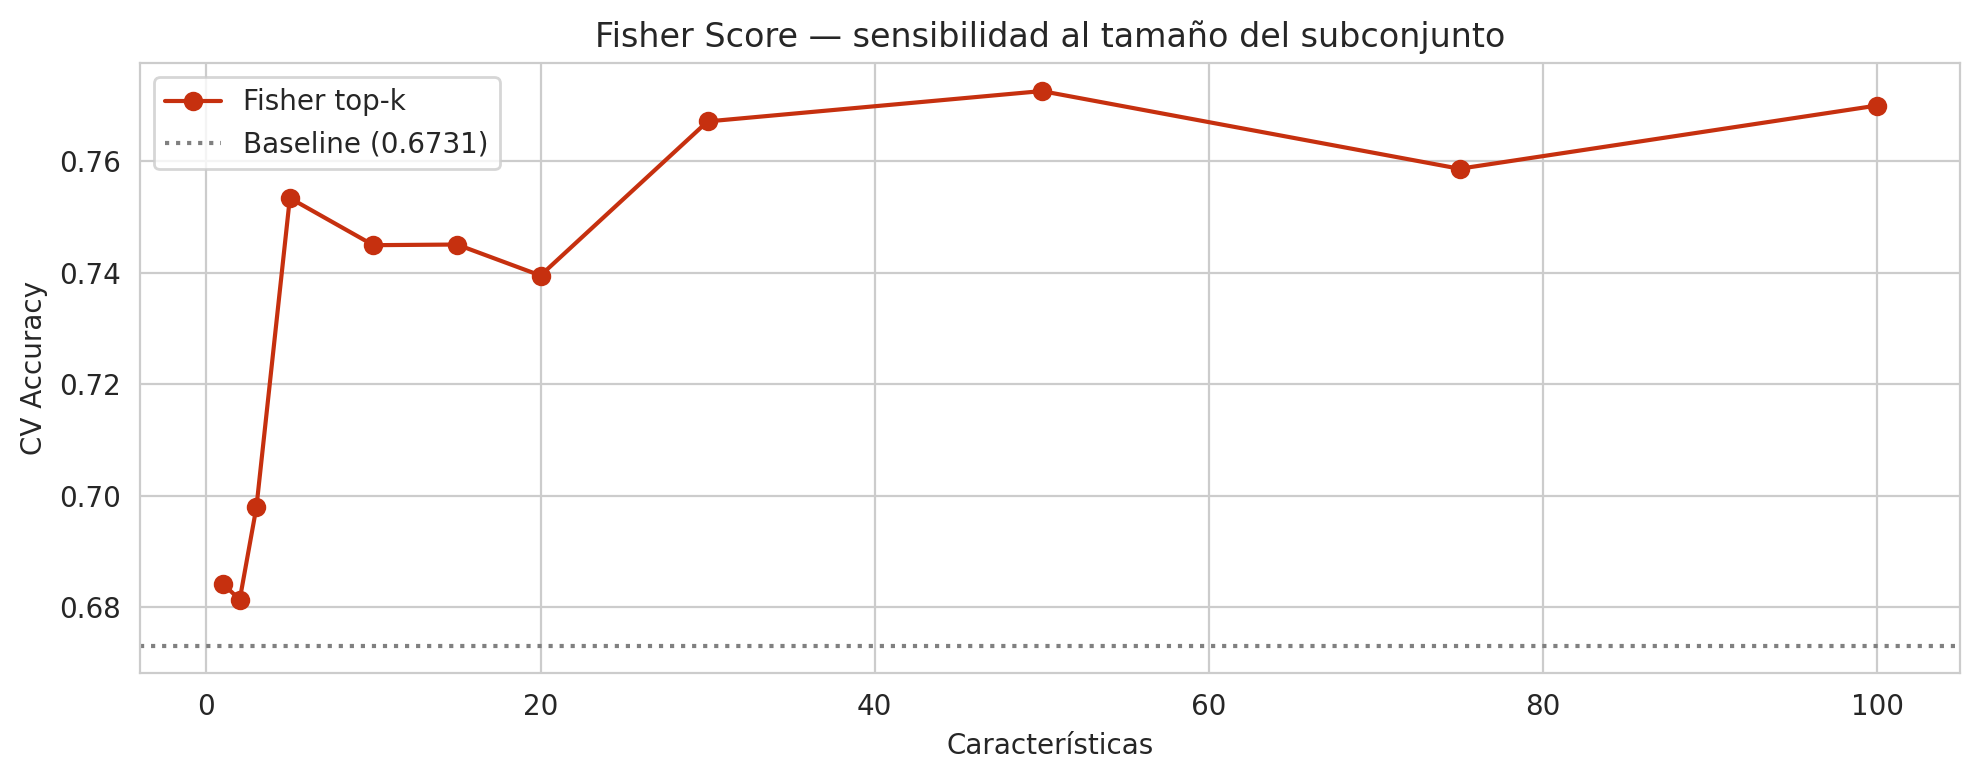
\includegraphics[width=0.85\textwidth]{Img/04_fisher_topk.png}
    \caption{Exactitud en CV en función del número de características top-$k$
        seleccionadas por Fisher Score.}
    \label{fig:fisher-topk}
\end{figure}

Usando las 20 mejores, la exactitud de CV fue $0.7395 \pm 0.0393$.

\subsubsection*{Análisis de Componentes Principales (PCA)}

Antes de aplicar PCA se eliminaron los pares de características con
correlación absoluta $|\rho| > 0.9$: esto removió 24 columnas,
dejando 237 para el análisis. Este paso es esencial porque PCA asume que la
varianza es proxy de información, y variables redundantes inflan
artificialmente los primeros componentes. El perfilamiento previo ya había
anticipado este problema al detectar pares altamente correlacionados entre
las 15 variables clínicas; al extender el análisis a las 261 columnas el
número de pares redundantes crece considerablemente.

La Figura~\ref{fig:pca-varianza} muestra la varianza acumulada. Son
necesarias \textbf{94 componentes} para alcanzar el $95\%$, lo que implica
que, pese a las 237 características de entrada, la información efectiva
ocupa aproximadamente ese número de dimensiones independientes. Con 94
componentes la exactitud de CV fue $0.6949 \pm 0.0841$.

\begin{figure}[H]
    \centering
    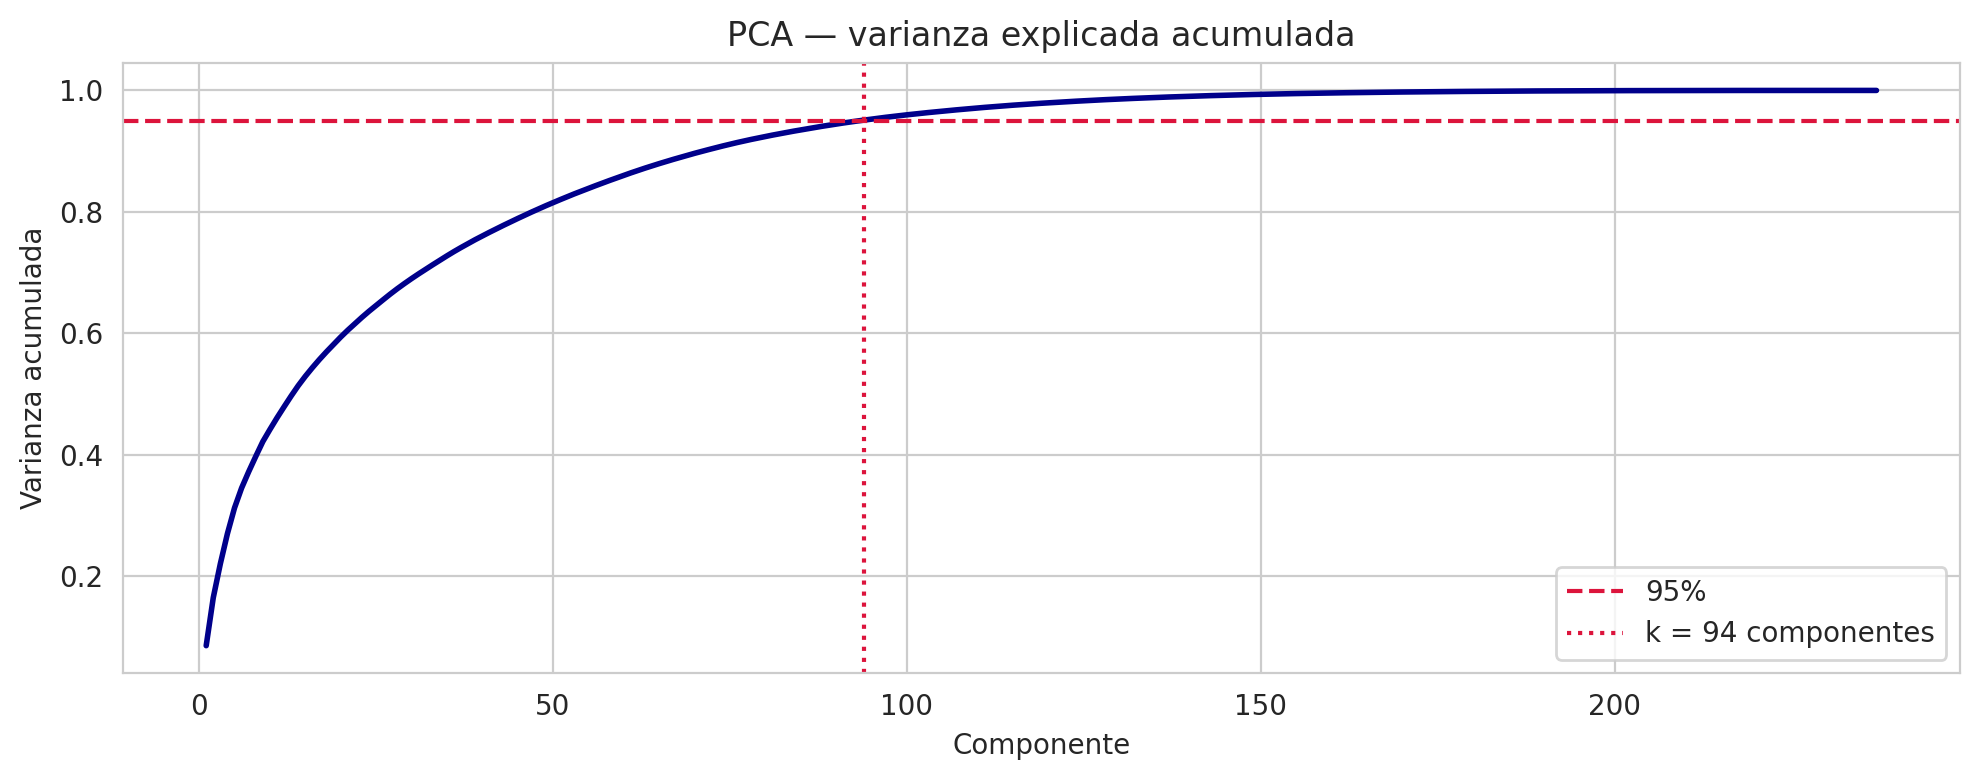
\includegraphics[width=0.85\textwidth]{Img/05_pca_varianza.png}
    \caption{Varianza explicada acumulada por PCA. Se requieren 94
        componentes para superar el umbral del $95\%$.}
    \label{fig:pca-varianza}
\end{figure}

La proyección sobre las dos primeras componentes (Figura~\ref{fig:pca-2d})
evidencia visualmente la dificultad del problema: ambas clases se
superponen extensamente en el plano PC1--PC2, que explica apenas un
$\sim 20\%$ de la varianza total. La falta de separación es esperable porque
PCA maximiza varianza, no discriminabilidad; las direcciones que más
separan normal de arritmia no tienen por qué coincidir con las de mayor
varianza.

\begin{figure}[H]
    \centering
    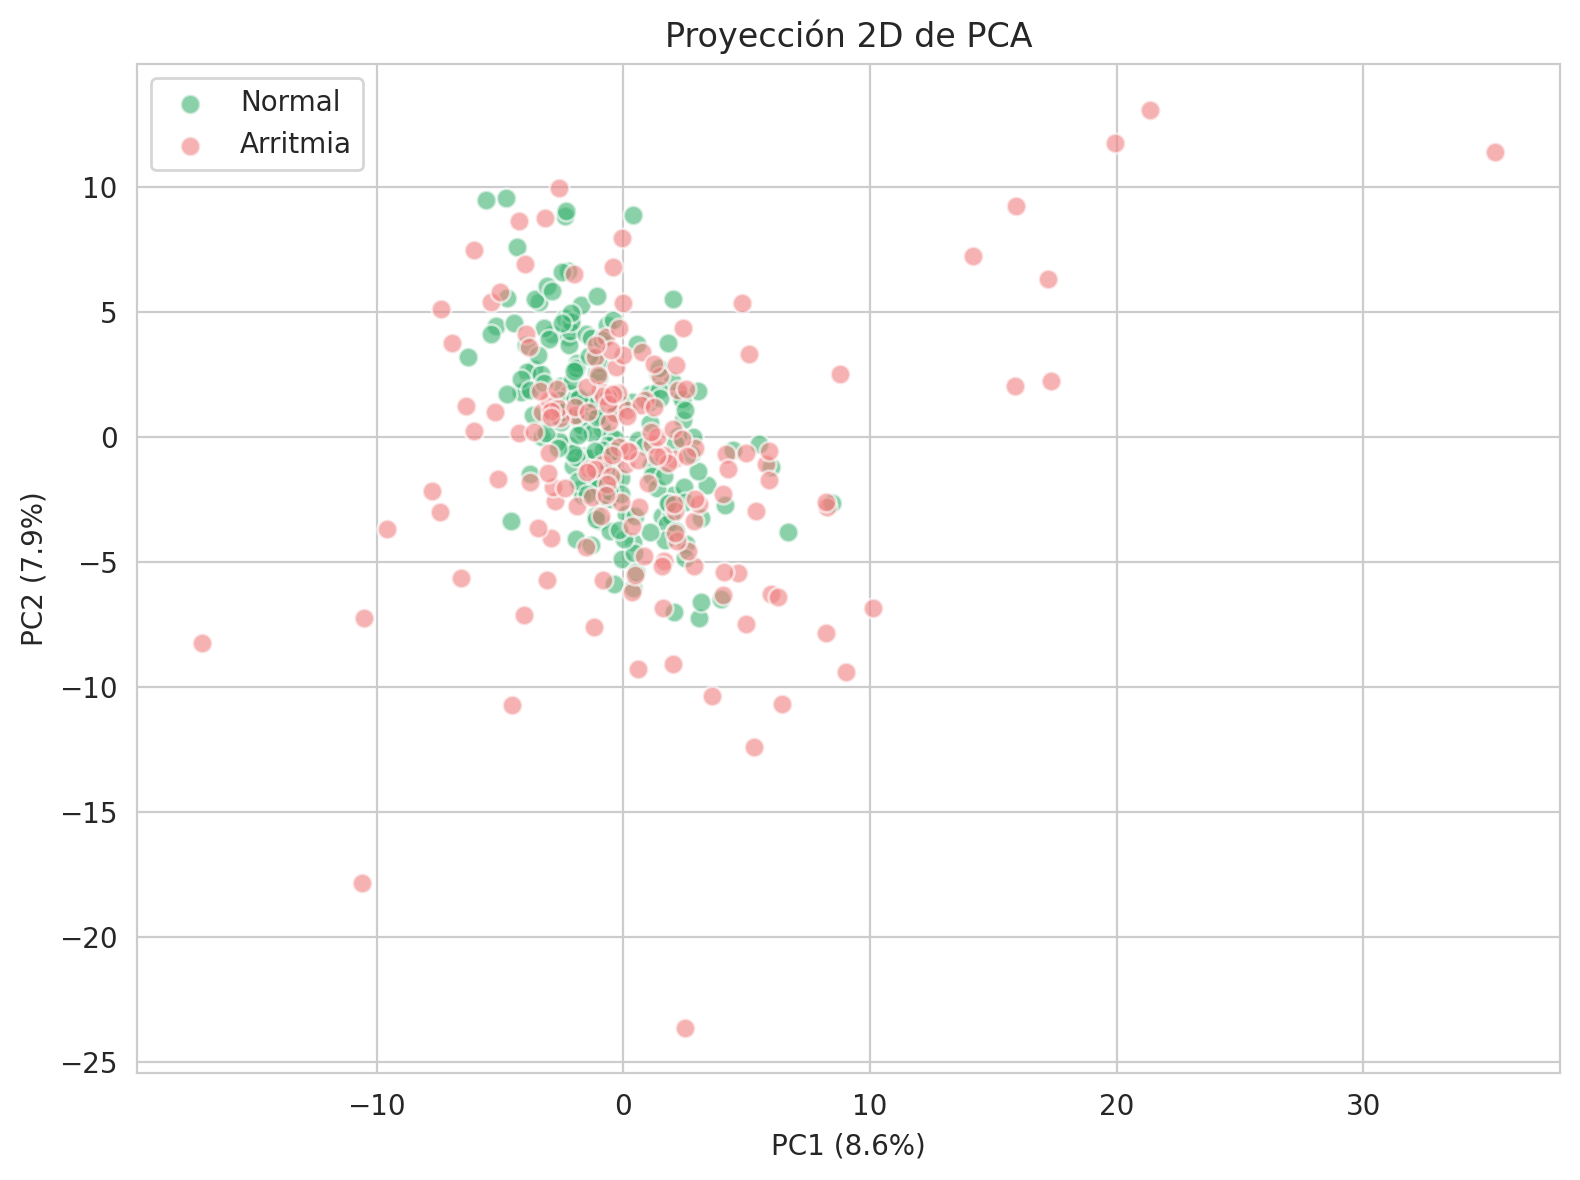
\includegraphics[width=0.75\textwidth]{Img/06_pca_2d.png}
    \caption{Proyección 2D de los datos de entrenamiento sobre las dos
        primeras componentes principales.}
    \label{fig:pca-2d}
\end{figure}

\subsection{Comparación final sobre el conjunto de prueba}

Con el subconjunto fijado por cada método se entrenó un SVM lineal sobre el
conjunto de entrenamiento completo y se evaluó sobre el $20\%$ de prueba,
intocado durante todo el proceso. La Tabla~\ref{tab:resultados} resume los
resultados y la Figura~\ref{fig:confusion} presenta las matrices de
confusión.

\begin{table}[H]
    \centering
    \rowcolors{2}{rowgray}{white}
    \begin{tabular}{lcccc}
        \toprule
        \rowcolor{headerblue}
        \textcolor{headertext}{\textbf{Método}}        &
        \textcolor{headertext}{\textbf{Nº feats}}      &
        \textcolor{headertext}{\textbf{CV Accuracy}}   &
        \textcolor{headertext}{\textbf{Test Accuracy}} &
        \textcolor{headertext}{\textbf{Test AUC}}                                                                               \\
        \midrule
        Baseline (todas)                               & 261        & $0.6731$          & $0.6484$          & $0.6905$          \\
        SFS manual                                     & 9          & $\mathbf{0.7782}$ & $0.7143$          & $0.7590$          \\
        SFS \texttt{sklearn}                           & \textbf{7} & $0.7755$          & $0.7143$          & $0.7585$          \\
        Fisher Score                                   & 20         & $0.7395$          & $\mathbf{0.7582}$ & $\mathbf{0.7638}$ \\
        PCA ($95\%$ var)                               & 94         & $0.6949$          & $0.6703$          & $0.6424$          \\
        \bottomrule
    \end{tabular}
    \caption{Comparativa de los métodos de selección de características.}
    \label{tab:resultados}
\end{table}

\begin{figure}[H]
    \centering
    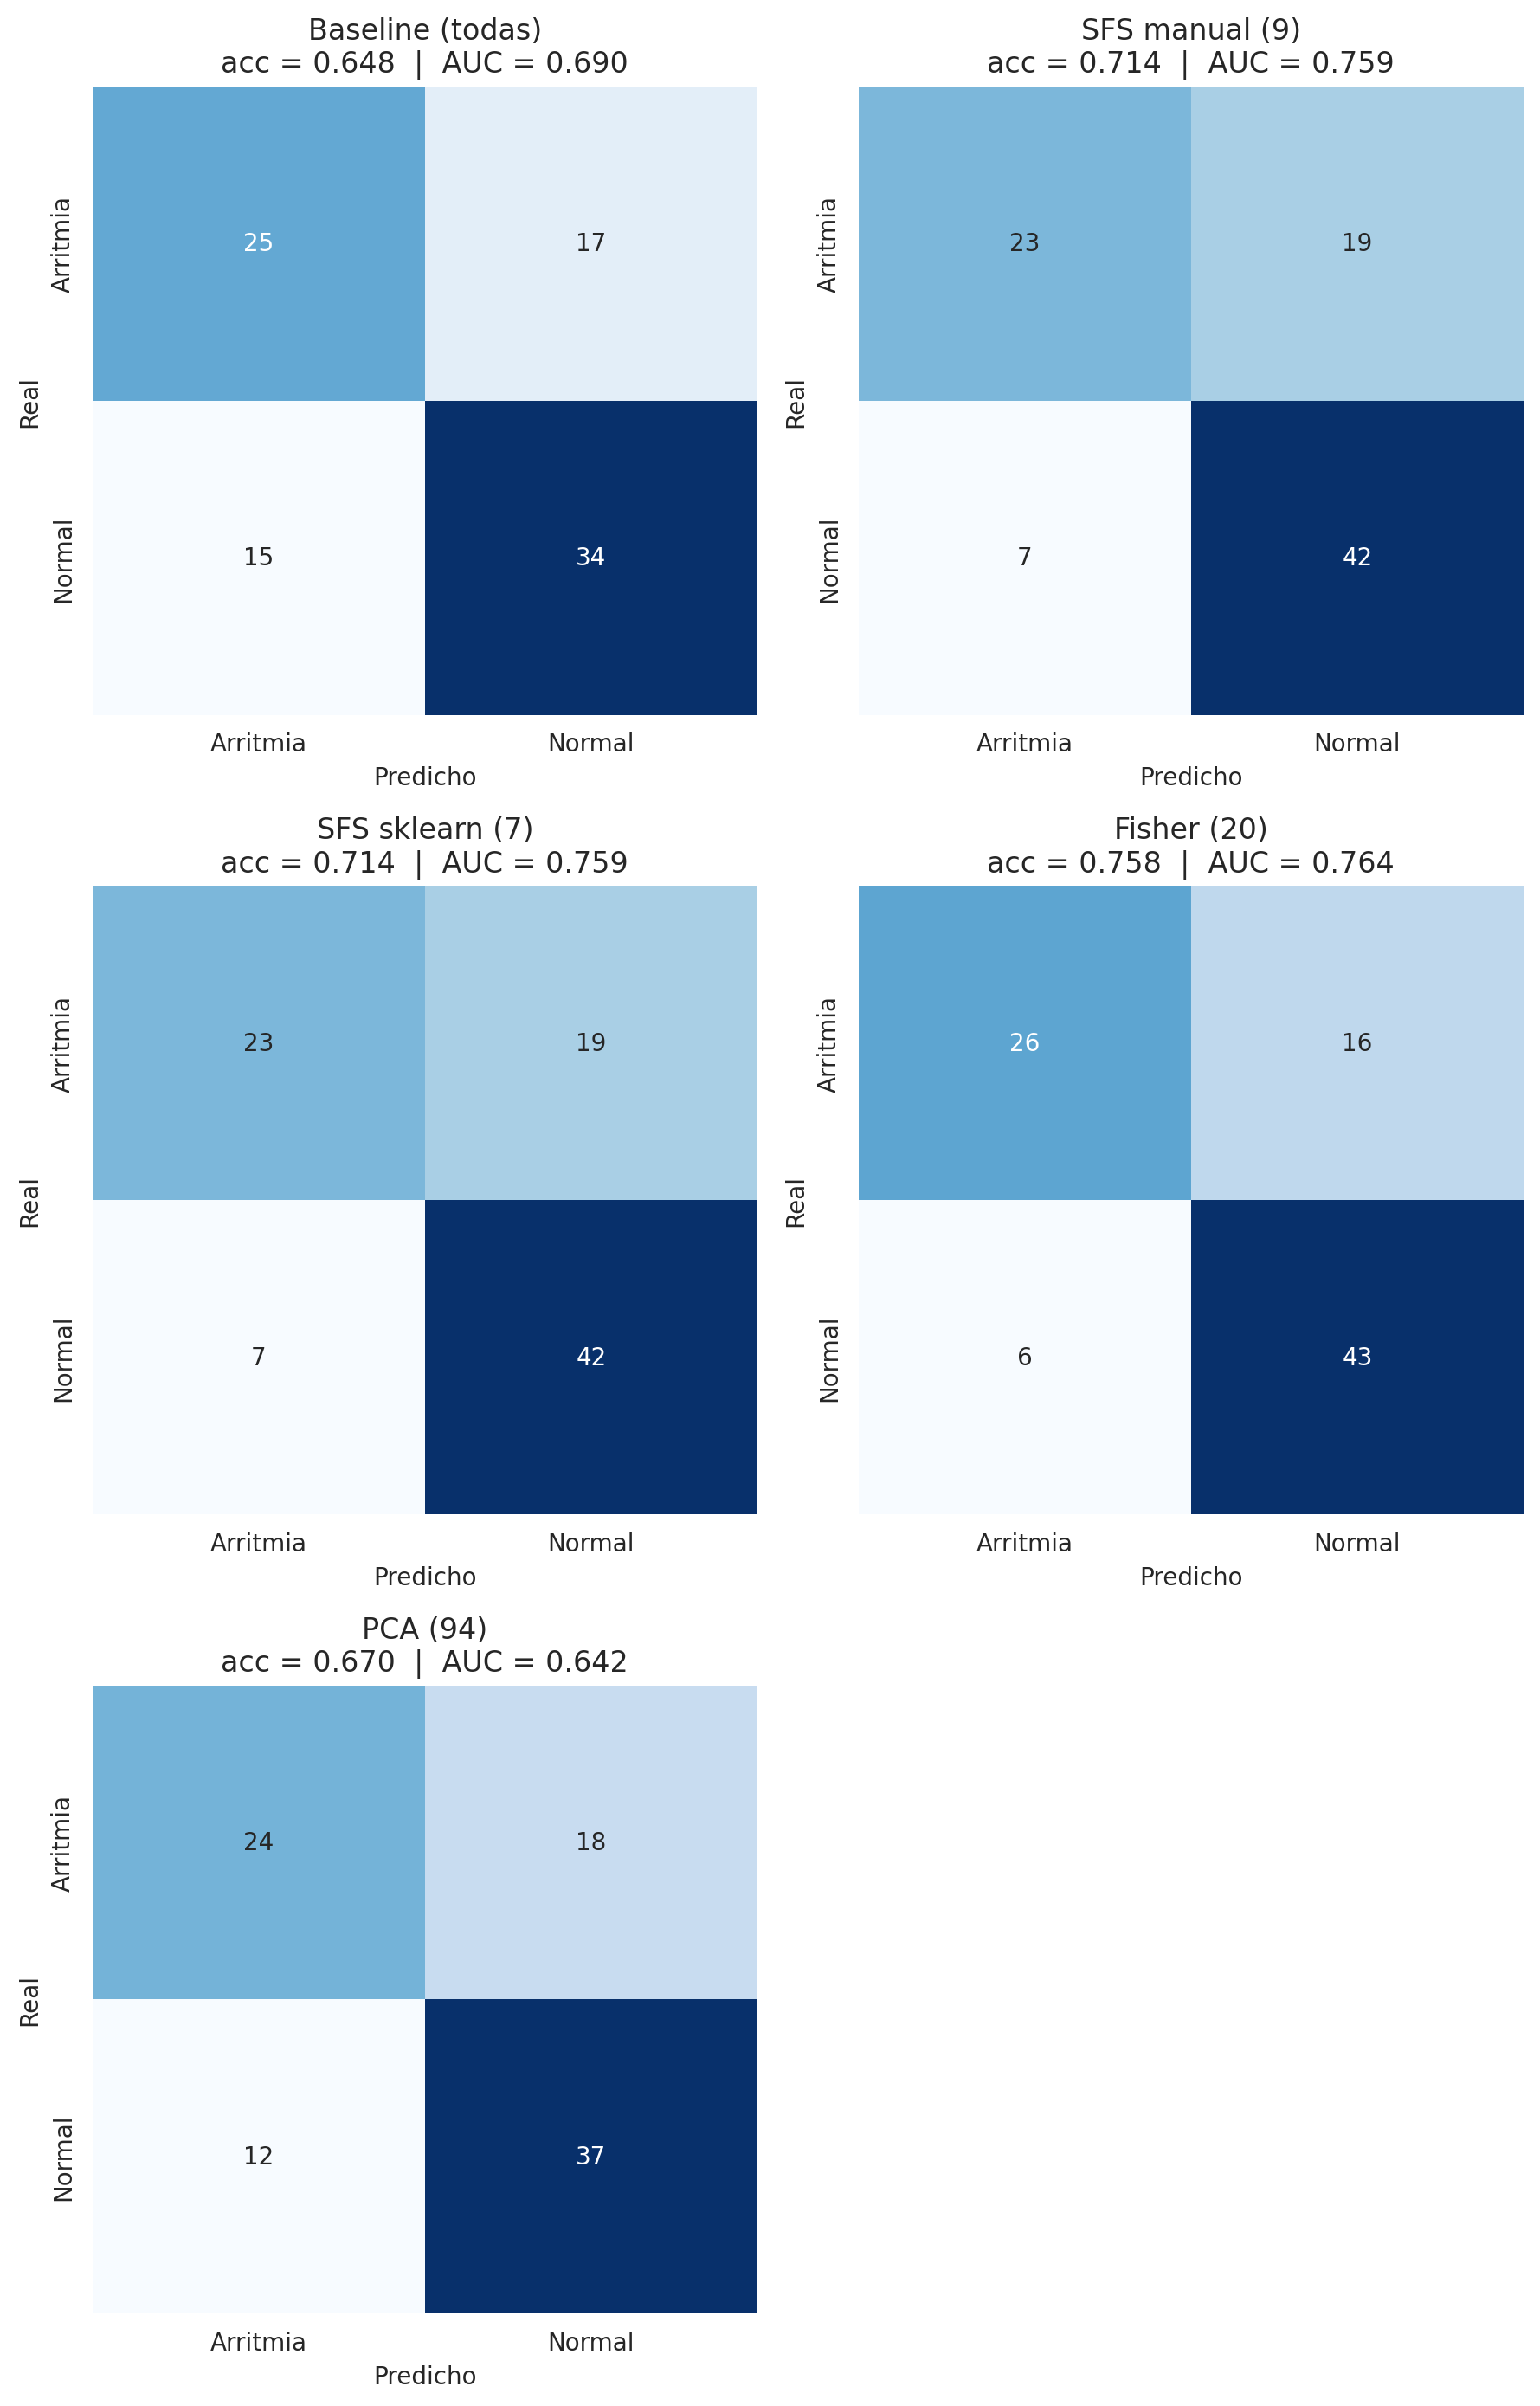
\includegraphics[width=0.77\textwidth]{Img/07_matrices_confusion.png}
    \caption{Matrices de confusión sobre el conjunto de prueba para cada
        método.}
    \label{fig:confusion}
\end{figure}

La intersección de las tres selecciones supervisadas (SFS manual, SFS
\texttt{sklearn} y Fisher Score) contiene exactamente
\texttt{qrs\_duration} y \texttt{a\_169}: son las dos candidatas que los
tres métodos coinciden en identificar como discriminantes.
\texttt{qrs\_duration} encabeza además el ranking de Fisher y es la
primera elegida por ambas versiones de SFS, confirmando su papel central.
Entre SFS manual y \texttt{sklearn} la coincidencia es incluso mayor, con
las 7 features de \texttt{sklearn} contenidas íntegramente en las 9 del
manual.

\subsection{Análisis de resultados}

\subsubsection*{(a) ¿Qué método obtuvo mejor exactitud? ¿Por qué?}

La respuesta depende de la métrica y del conjunto donde se mida:

\begin{itemize}
    \item En \textbf{validación cruzada}, las dos versiones de SFS fueron
          superiores (manual $0.7782$, \texttt{sklearn} $0.7755$), seguidas
          por Fisher ($0.7395$) y PCA ($0.6949$). Es el resultado esperado:
          SFS es un método \textit{wrapper} que optimiza directamente la
          métrica del clasificador final y captura interacciones entre
          variables.

    \item En \textbf{prueba}, sin embargo, \textbf{Fisher Score} obtuvo la
          mejor exactitud ($0.7582$) y la mejor AUC ($0.7638$), mientras
          que ambas versiones de SFS quedaron ligeramente por debajo
          ($0.7143$ en exactitud). La diferencia entre CV y test ---de
          $0.778$ a $0.714$ en SFS manual--- es un caso clásico de
          \textit{selection bias}: al buscar exhaustivamente en el
          espacio de subconjuntos usando la misma CV, el método
          sobreajusta y el optimismo no se traslada al conjunto de
          prueba. Fisher, al ser un filtro que no optimiza la métrica del
          clasificador, es menos vulnerable a ese sesgo.
\end{itemize}

Un punto metodológico importante: el tamaño del conjunto de prueba es de
apenas 91 muestras, por lo que una diferencia de $4$ puntos porcentuales
está dentro del ruido muestral. Los AUC de los tres métodos supervisados
($0.7585$--$0.7638$) son prácticamente indistinguibles. Concluir que
Fisher ``gana'' de forma categórica sería precipitado; lo honesto es decir
que los tres métodos son equivalentes en generalización y que SFS paga su
mejor ajuste en CV con una ligera pérdida en test.

\subsubsection*{(b) ¿Qué método es más robusto ante outliers y desbalanceo?}

\textbf{Fisher Score} es el más robusto frente al desbalanceo porque
pondera explícitamente por $n_c$ (véase la ecuación~\ref{eq:fisher}) y
trabaja con estadísticos por clase, no con una métrica global que pueda
sesgarse hacia la clase mayoritaria. SFS con exactitud como criterio es el
más vulnerable: si una clase domina, la métrica puede recompensar
predicciones triviales.

Frente a \textit{outliers}, ninguno de los tres es intrínsecamente robusto:
tanto Fisher como PCA dependen de medias y varianzas, que son sensibles a
valores extremos. El escalado \textit{z-score} aplicado previamente
limita la escala de los outliers, pero para robustez genuina convendría
usar variantes basadas en mediana/MAD o PCA robusto.

\subsubsection*{(c) ¿Cómo afecta la correlación entre características al PCA?}

PCA identifica las direcciones de máxima varianza. Cuando dos o más
variables están fuertemente correlacionadas representan esencialmente la
misma dirección en el espacio de características, pero su varianza se
acumula en ese eje, haciéndolo parecer más relevante de lo que
efectivamente es. En consecuencia, los primeros componentes capturan
información redundante en vez de independiente, degradando la capacidad
del método para comprimir el dataset.

En este trabajo el perfilamiento exploratorio ya alertó sobre pares
fisiológicamente redundantes como \texttt{heart\_rate}--\texttt{qt\_interval}
o \texttt{qrs\_angle}--\texttt{qrst\_angle}, que son un caso claro del
problema: miden fenómenos relacionados por construcción. Al extender el
filtro $|\rho|>0.9$ sobre las 261 columnas se eliminaron 24 antes de
aplicar PCA. Sin ese filtro, se habrían necesitado más componentes para
llegar al $95\%$ de varianza, pues los primeros componentes estarían
dominados por bloques de variables casi duplicadas.

\subsubsection*{(d) ¿Qué ventajas tiene Fisher Score sobre SFS en términos computacionales?}

La diferencia es de varios órdenes de magnitud. Fisher Score tiene
complejidad $\mathcal{O}(n \cdot d)$: un solo recorrido de los datos
calculando medias y varianzas por clase, enteramente vectorizable. SFS,
en cambio, es $\mathcal{O}(d^2 \cdot k_{cv} \cdot t_{fit})$: en cada una
de sus iteraciones entrena el clasificador una vez por cada característica
candidata restante, con validación cruzada completa.

En esta práctica, SFS ---tanto la versión manual como la de
\texttt{sklearn}--- necesitó entrenar del orden de $15{,}000$ modelos
SVM, tardando alrededor de un minuto en un equipo moderno; Fisher se
calculó en milisegundos. Esta diferencia explica por qué Fisher y sus
parientes (\textit{mutual information}, F-ANOVA, $\chi^2$) son el
estándar en problemas de ultra-alta dimensionalidad como los de genómica
(p.~ej. el dataset de Golub con 7129 genes), donde SFS sería directamente
inviable sin paralelización agresiva o recorte previo del espacio de
búsqueda.

El hecho de que, \emph{en este dataset concreto}, Fisher no sólo sea
mucho más rápido sino que además generalice mejor al conjunto de prueba
que SFS ilustra que la ventaja computacional no siempre va aparejada a
una pérdida de calidad. Una estrategia pragmática sería usar Fisher como
filtro inicial y SFS únicamente sobre el subconjunto resultante cuando la
dimensionalidad original sea prohibitiva.
